\documentclass[letterpaper,12pt]{article}
\usepackage[utf8]{inputenc}
\usepackage[russian]{babel}
\usepackage[left=2cm,right=2cm,top=2cm,bottom=2cm,bindingoffset=0cm]{geometry}
\usepackage{graphicx}
\graphicspath{{images/}}
\usepackage{float}
\usepackage{wrapfig}

\begin{document}

\begin{center}
      Алгоритм определения правильности отрезка.
\end{center}

Входные данные: отрезок $s$, грань РСДС $f$, упорядоченное по 
полярному углу множество точек $P_u$, индексы $i, j$ краевых точек $s$
в $P_u$.

Выходные данные: <<да>>, если $s$ правильный. <<нет>>, если $s$ 
неправильный. 

Алгоритм: если $i \neq (j \pm 1) \ mod \ n-1$, то ответ <<нет>>. Иначе 
выбираем произвольную внутреннюю точку $f$ (например середина прямой, 
соединяющей середины любых двух соседних ребер), находим ориентированную
площадь треугольника $p_i q p_j$ (Не умаляя общности, считаем что 
$i = (j - 1) \ mod \ n-1$), если она положительна, то ответ <<да>>, иначе
ответ <<нет>>.

\begin{center}
Описание случаев поведения алгоритма в процессе <<перешагивания>> ребра
\end{center}
Содержание статуса: 
\begin{enumerate}
      \item Упорядоченные по полярному углу точки отрезков.
      \item Информация о правильности всех отрезков.
      \item Информация о порядке точек внутри отрезков.
\end{enumerate}

На каждом шаге важным является константный доступ к затрагиваемым
отрезкам, информации об их правильности, внутреннем порядке точек.

Не умаляя общности, рассмотрим случаи для ребра расположенного вертикально:
\begin{enumerate}
      \item Точки $p_i, p_j$ являются точками одного отрезка. 
            Так как перешагивание отрезка исключено из рассмотрения,
            возможен только вариант представленный ниже, а также
            зеркальный к нему.

            \begin{figure}[h]
                  \centering
                  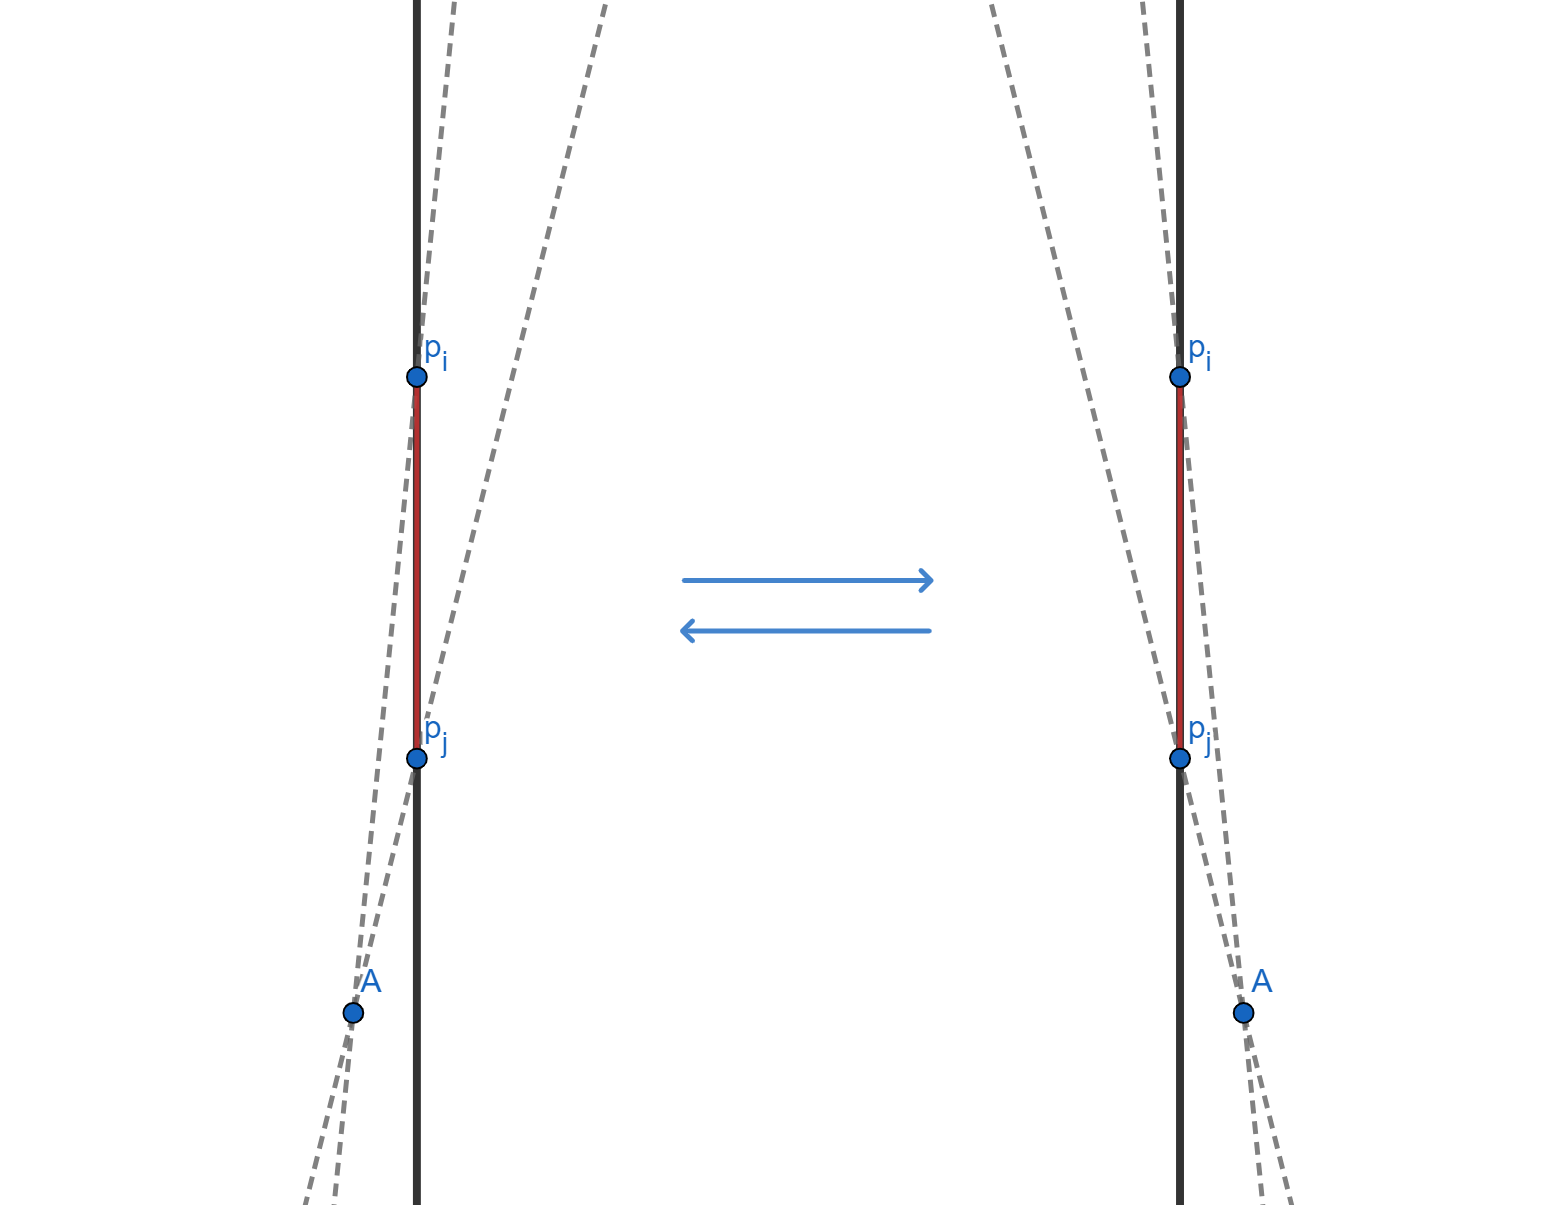
\includegraphics[width=.5\linewidth]{one_segment_1.png}
            \end{figure}

      \item Точки $p_i, p_j$ лежат на прямой с одной стороны относительно
            <<перешагиваемого>> ребра. Возможны варианты, изображенные ниже,
            а также зеркальные к ним.

            Выбор какую из точек выбрать за $p_i$ неважен.

            \begin{figure}[H]
                  \centering
                  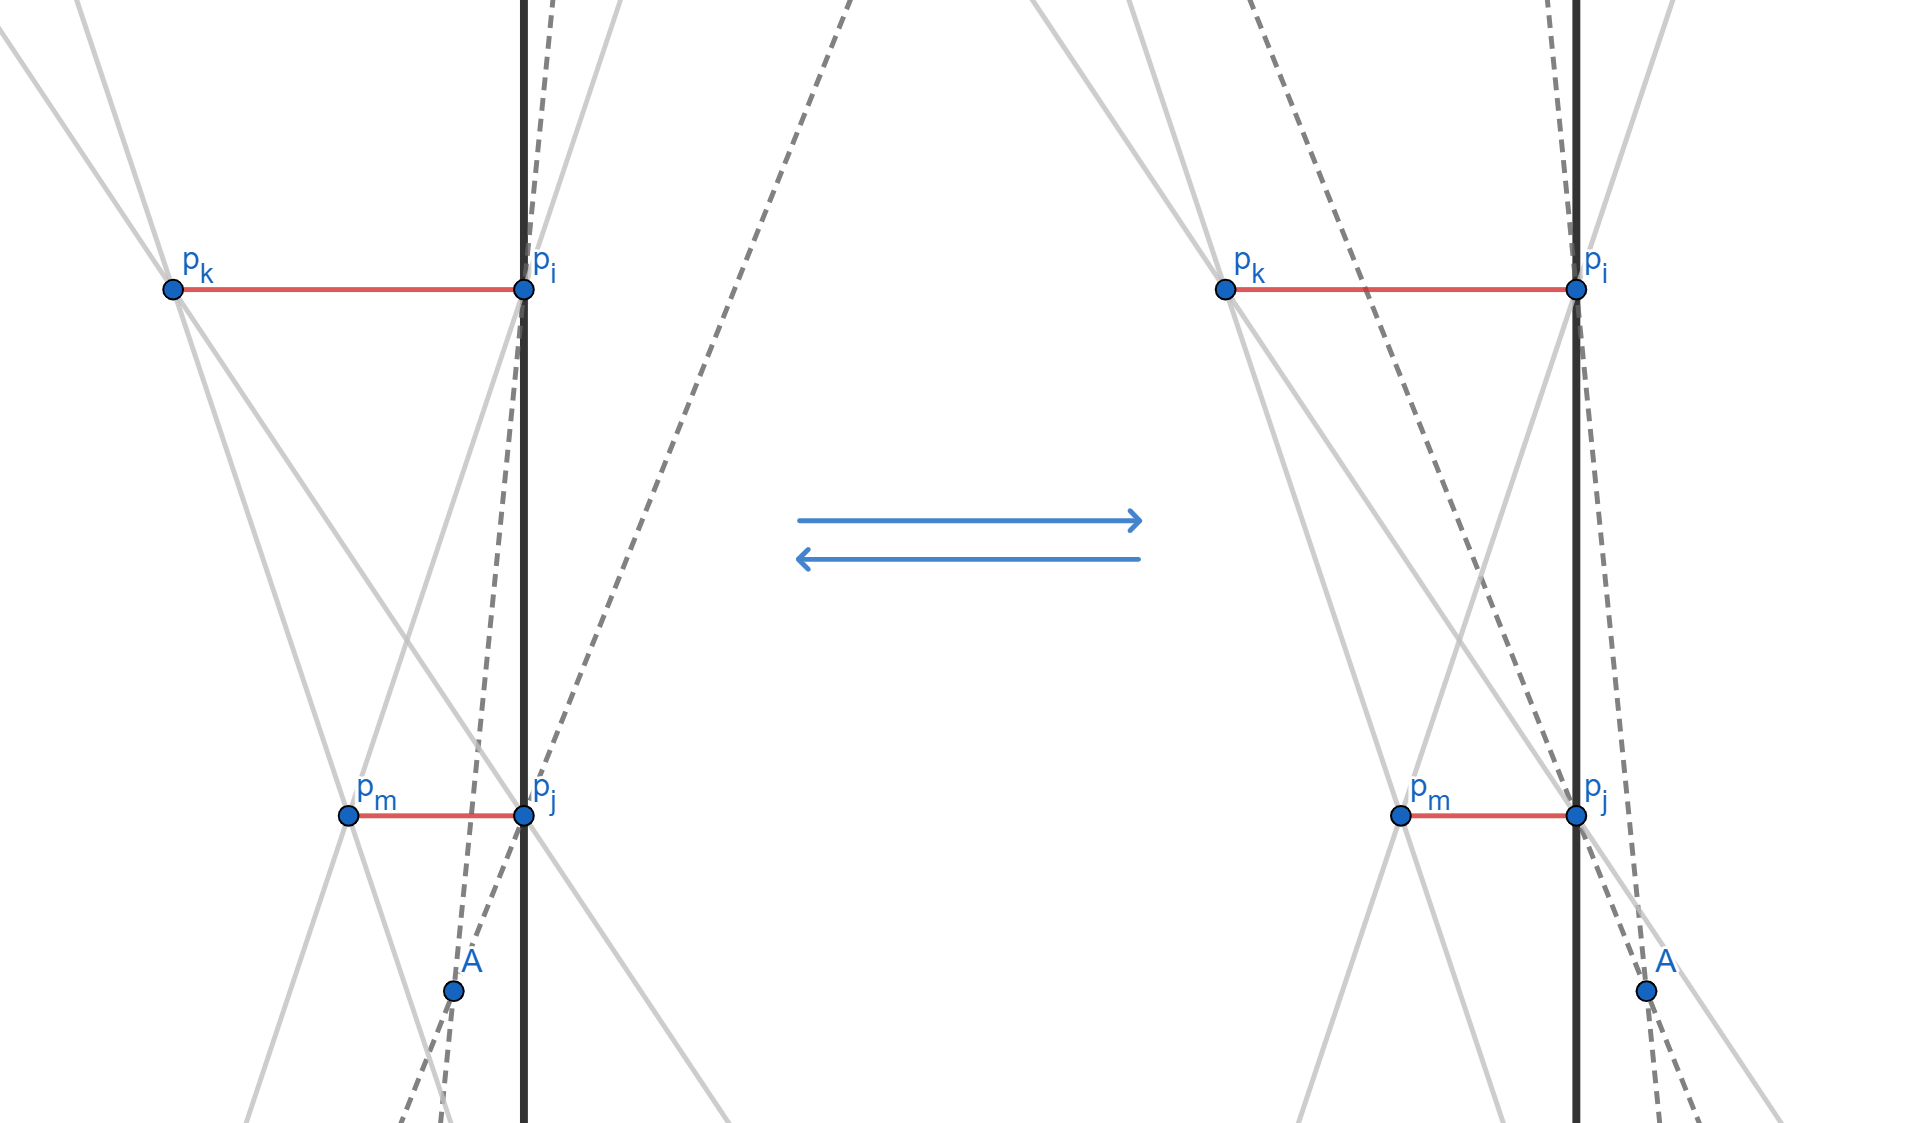
\includegraphics[width=.6\linewidth]{one_side_1.png}
            \end{figure}

            \begin{figure}[H]
                  \centering
                  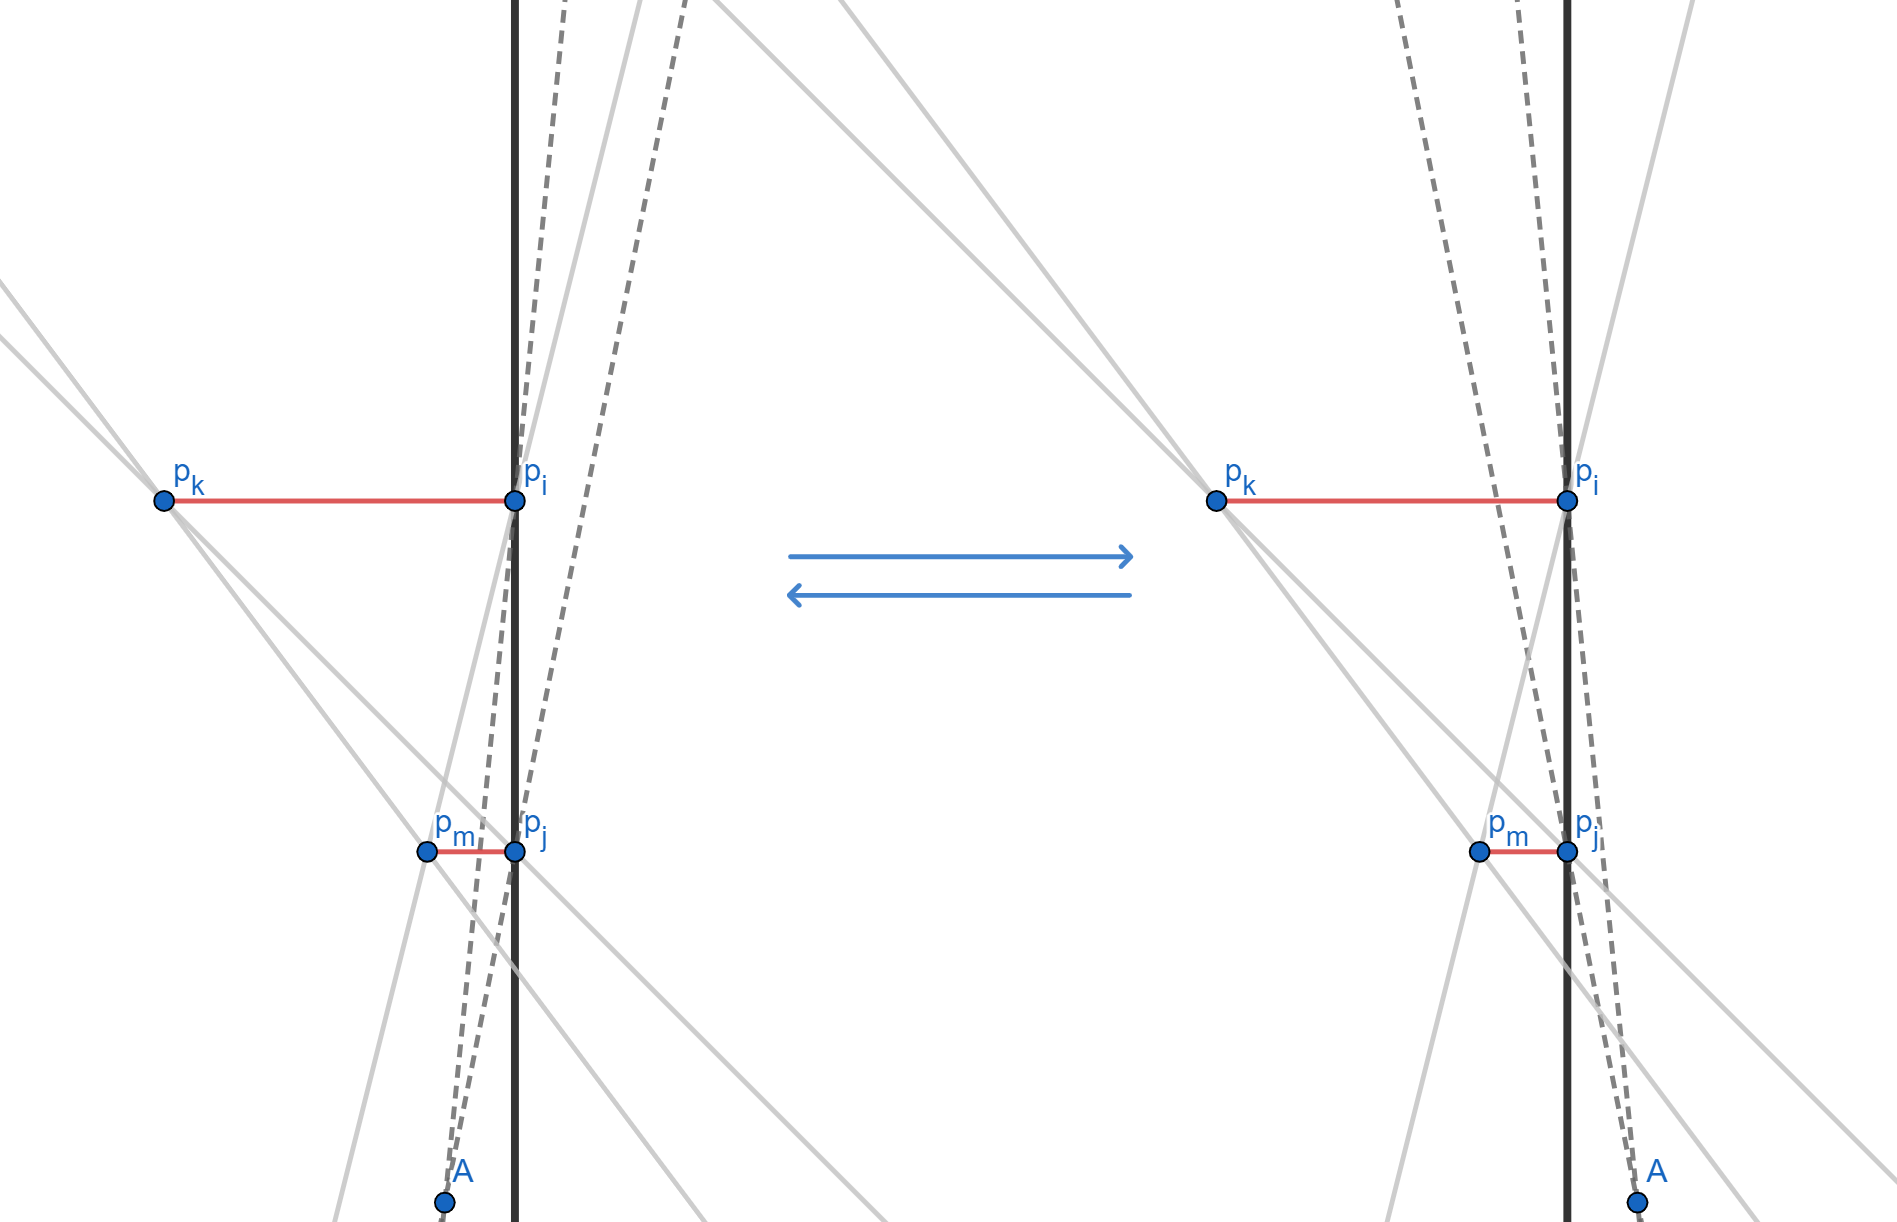
\includegraphics[width=.6\linewidth]{one_side_3.png}
            \end{figure}

            \begin{figure}[H]
                  \centering
                  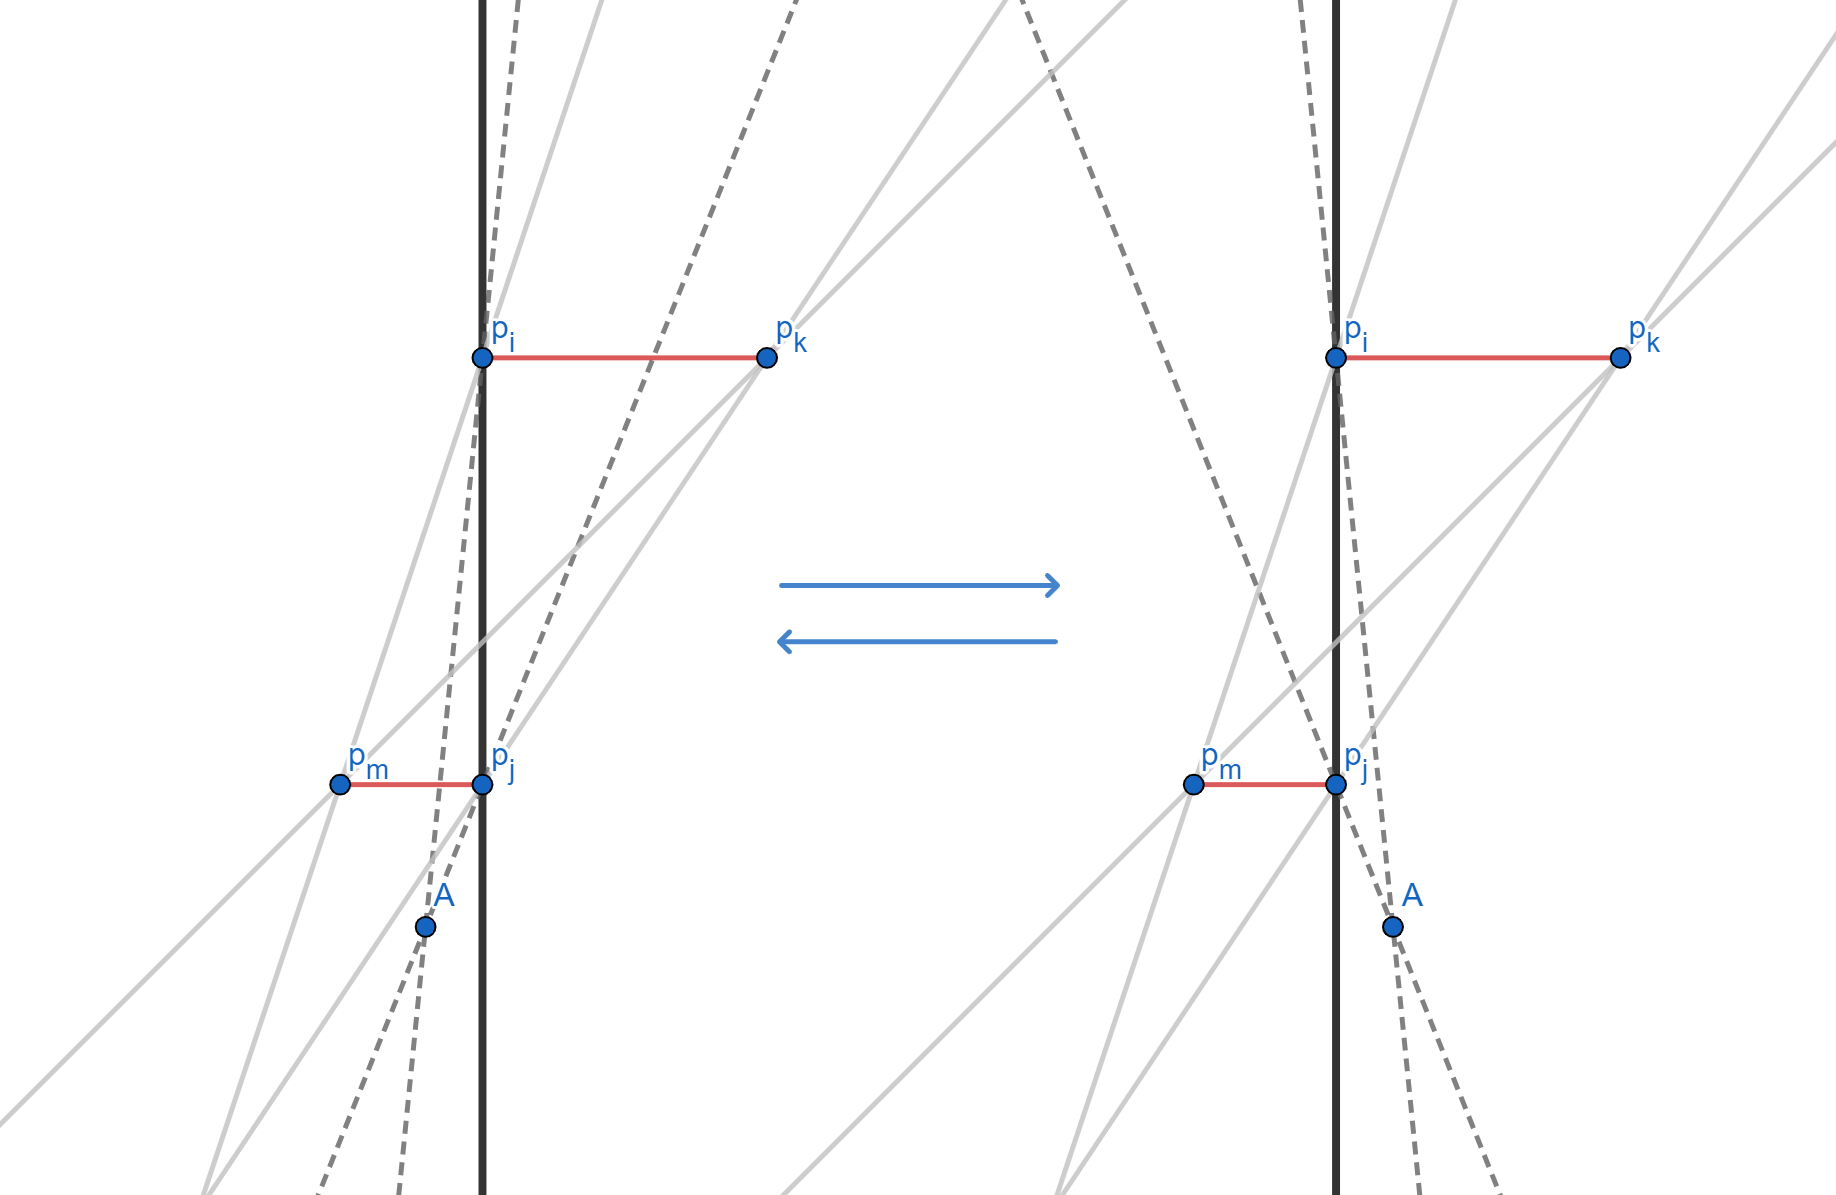
\includegraphics[width=.6\linewidth]{one_side_2.png}
            \end{figure}

            \begin{figure}[H]
                  \centering
                  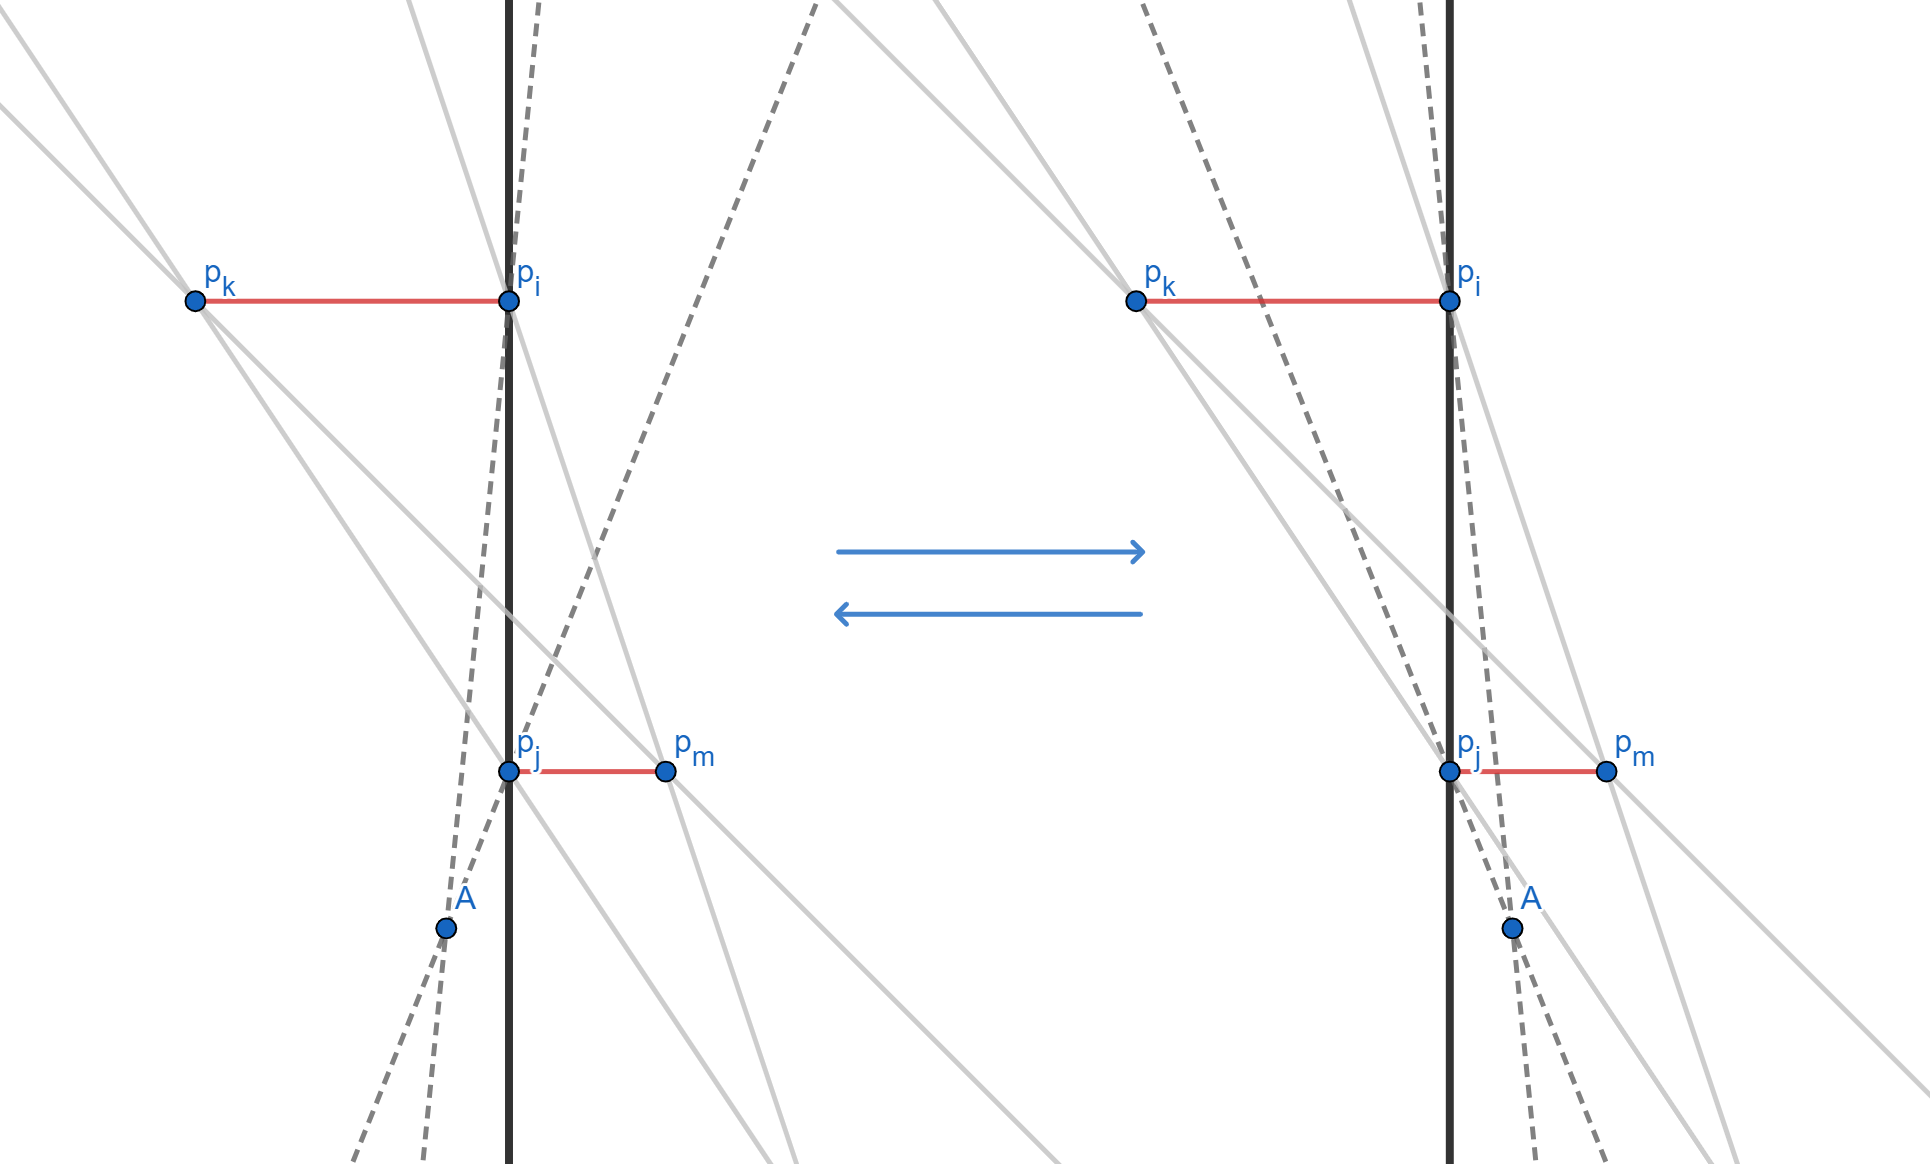
\includegraphics[width=.6\linewidth]{one_side_4.png}
            \end{figure}

      \item Точки $p_i, p_j$ лежат на прямой по разные стороны 
            относительно <<Перешагиваемого>> ребра. Возможны варианты, 
            изображенные ниже, а также зеркальные к ним.

            \begin{figure}[H]
                  \centering
                  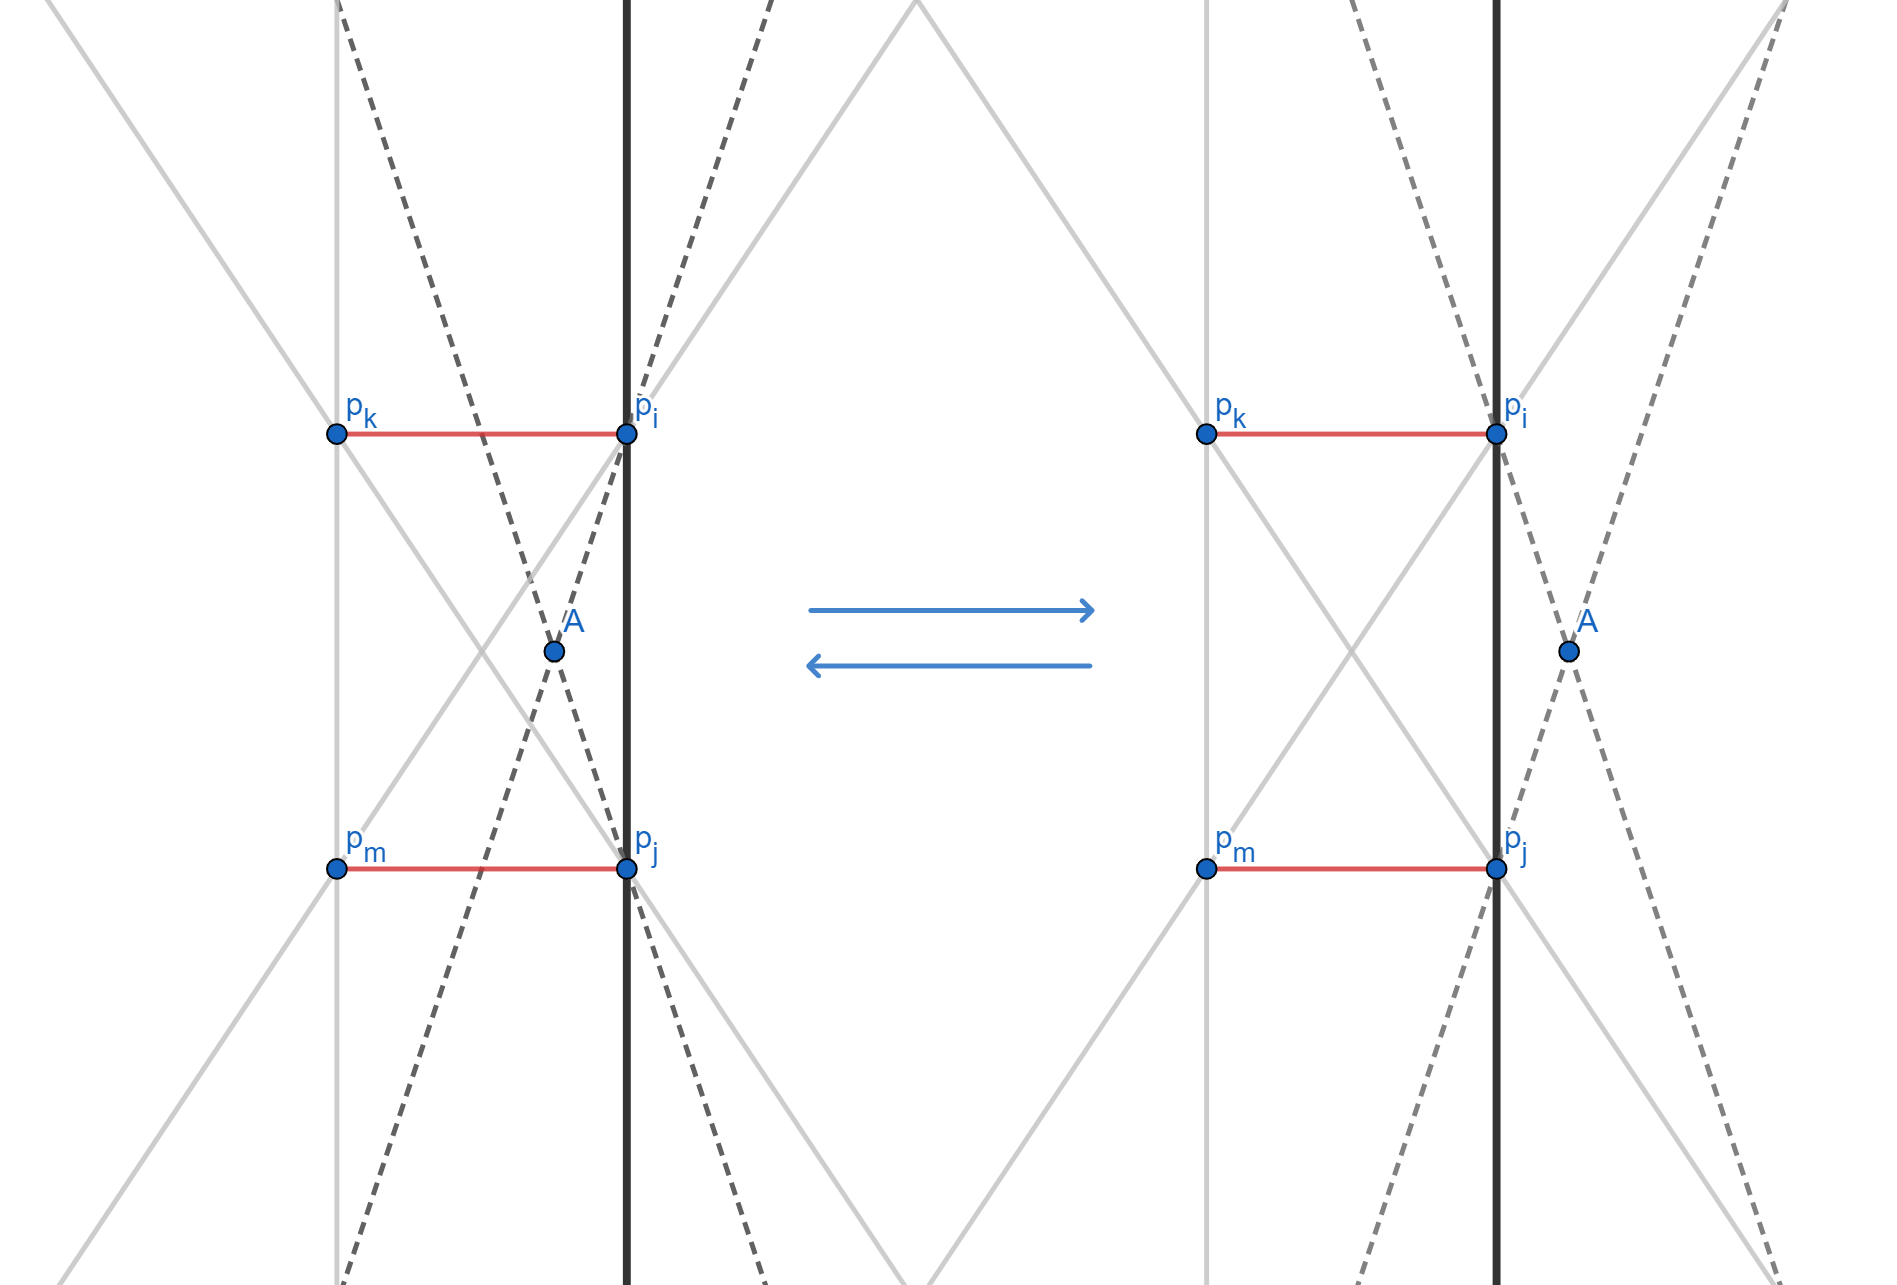
\includegraphics[width=.6\linewidth]{between_1.png}
            \end{figure}

            \begin{figure}[H]
                  \centering
                  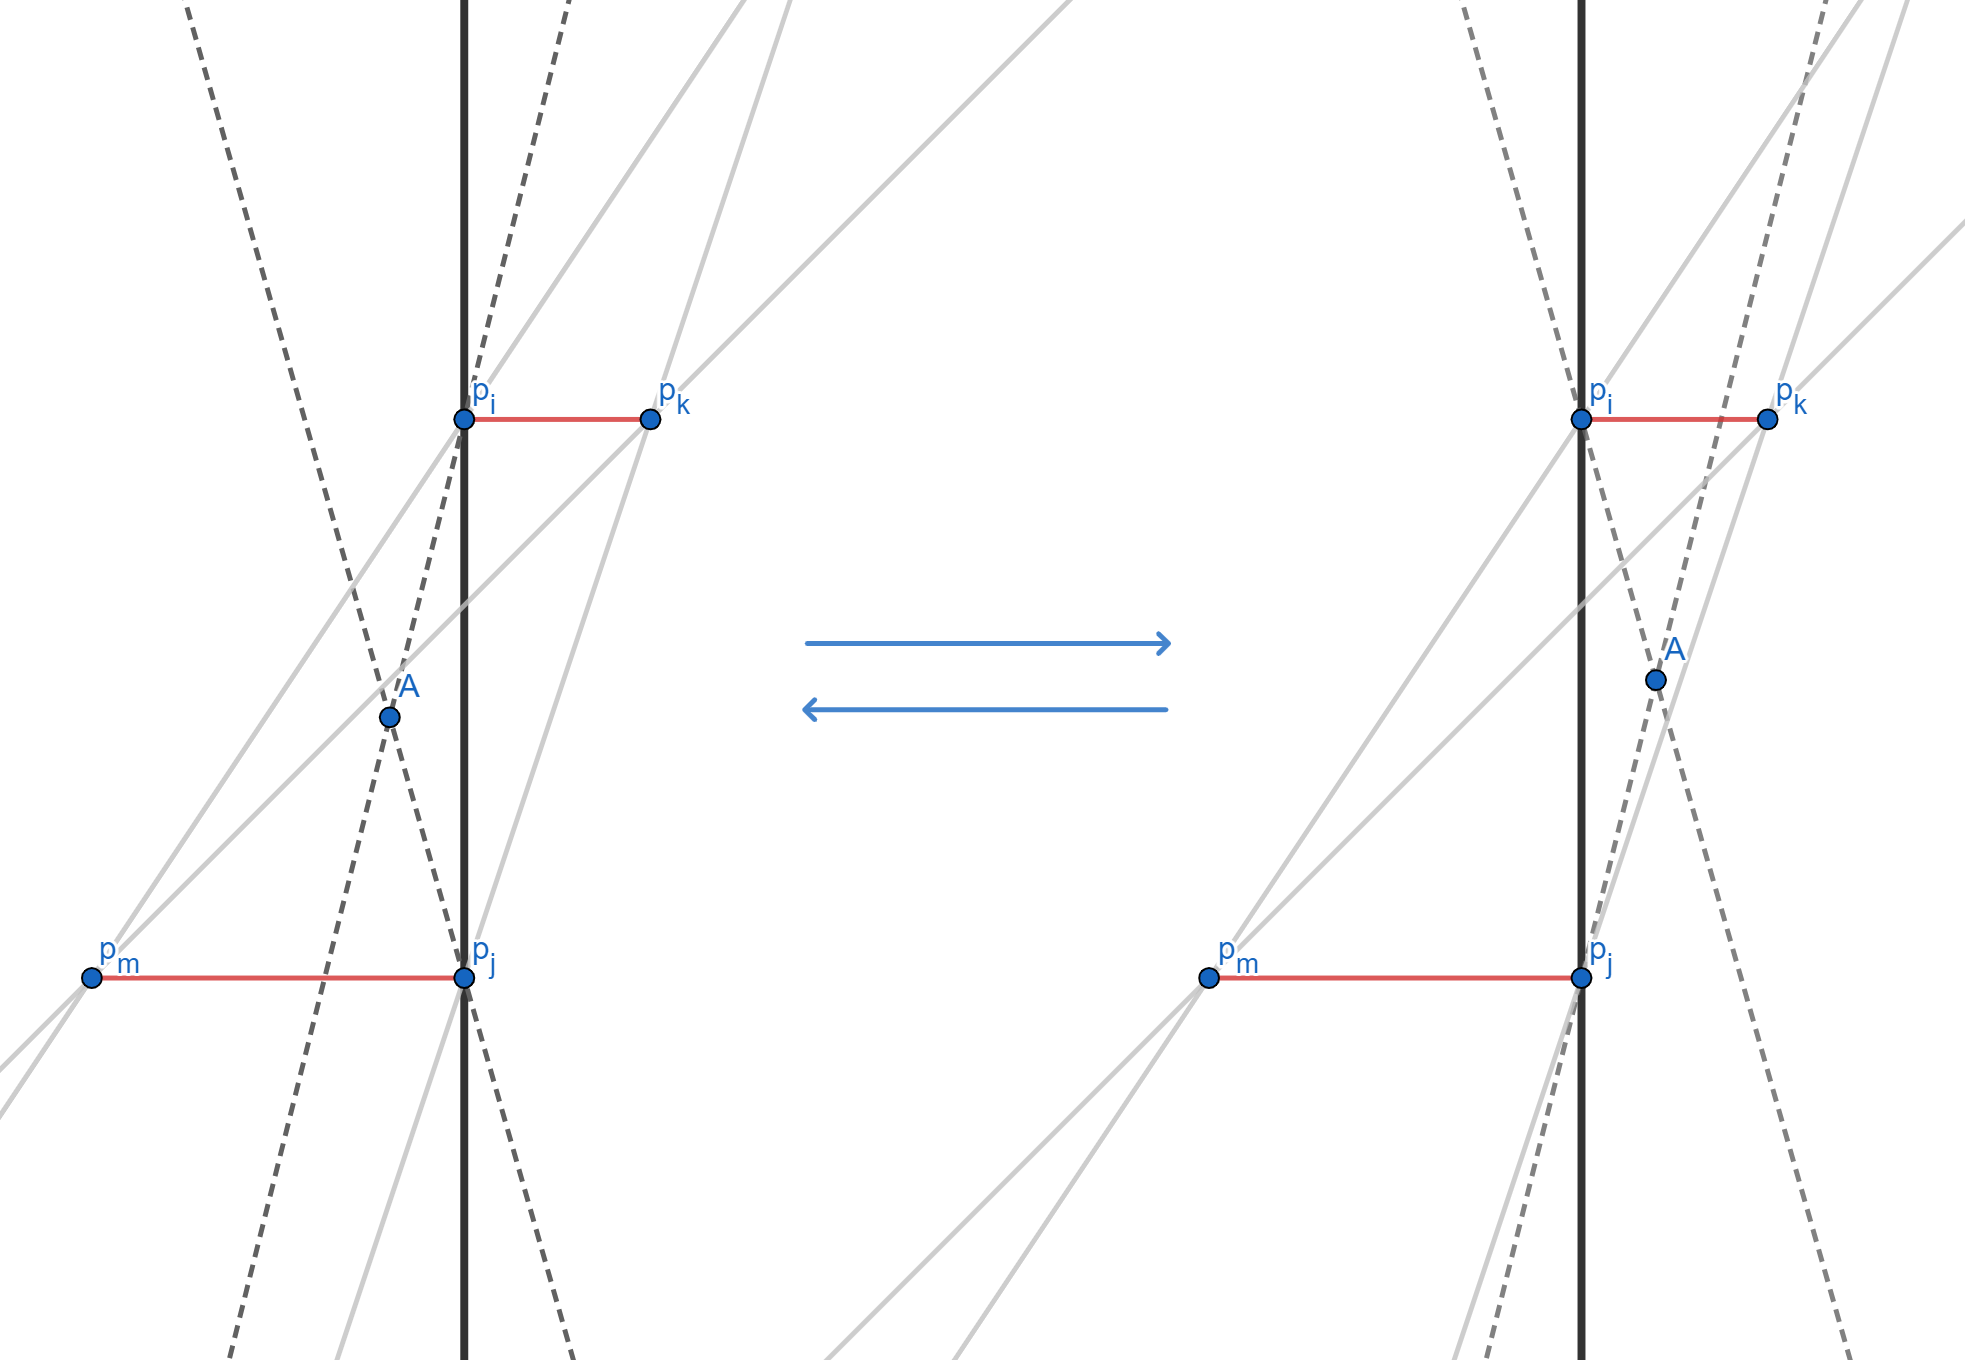
\includegraphics[width=.6\linewidth]{between_2.png}
            \end{figure}
\end{enumerate}

Таблицы изменений статуса для каждого случая.

Случаи разбиты на пары (по сути "до-после").

Последние 2 пары выделены отдельно. 6 пару можно определить
однозначно только если держать в ребре информацию об относительном 
положении порождающих его точек (с одной стороны/с разных сторон).

Правильность: $+$ - правильный, $-$ - неправильный,
$?$ - если точки рядом, то правильный.

\begin{center}
      \begin{tabular}{| c | c | c | c |}
            \hline
            номер & порядок в массиве & 
            правильность & порядок в отрезке \\
            \hline
            $1.1$ &
            $..., p_j, p_i, ...$ & $+$ & $p_j, p_i$ \\
            \hline
            $1.2$ &
            $..., p_i, p_j, ...$ & $+$ & $p_i, p_j$ \\
            \hline
            $2.1$ &
            $p_j, ..., p_i, ..., p_k, ..., p_m$ & 
            $?$, $-$ & $p_i, p_k$ : $p_j, p_m$ \\
            \hline
            $2.2$ &
            $p_i, ..., p_j, ..., p_k, ..., p_m$ & 
            $-$, $-$ & $p_i, p_k$ : $p_j, p_m$ \\
            \hline
            $3.1$ &
            $p_j, ..., p_i, ..., p_m, ..., p_k$ & 
            $-$, $-$ & $p_i, p_k$ : $p_j, p_m$ \\
            \hline
            $3.2$ &
            $p_i, ..., p_j, ..., p_m, ..., p_k$ & 
            $?$, $-$ & $p_i, p_k$ : $p_j, p_m$ \\
            \hline
            $4.1$ &
            $p_j, ..., p_i, ..., p_m, ..., p_k$ & 
            $-$, $-$ & $p_k, p_i$ : $p_j, p_m$ \\
            \hline
            $4.2$ &
            $p_i, ..., p_j, ..., p_m, ..., p_k$ & 
            $?$, $?$ & $p_k, p_i$ : $p_j, p_m$ \\
            \hline
            $5.1$ &
            $p_j, ..., p_i, ..., p_k, ..., p_m$ & 
            $?$, $?$ & $p_i, p_k$ : $p_m, p_j$ \\
            \hline
            $5.2$ &
            $p_i, ..., p_j, ..., p_k, ..., p_m$ & 
            $-$, $-$ & $p_i, p_k$ : $p_m, p_j$ \\
            \hline    
      \end{tabular}
\end{center}

\begin{center}
      \begin{tabular}{| c | c | c | c |}
            \hline
            порядок в массиве & правильность &
            порядок в отрезке \\
            \hline
            $6.1$ &
            $p_j, ..., p_i, ..., p_k, ..., p_m$ &
            $?$, $?$ & $p_i, p_k$ : $p_m, p_j$ \\
            \hline
            $6.2$ &
            $p_j, ..., p_i, ..., p_k, ..., p_m$ &
            $?$, $?$ & $p_i, p_k$ : $p_m, p_j$ \\
            \hline
            $7.1$ &
            $p_j, ..., p_k, ..., p_i, ..., p_m$ &
            $?$, $?$ & $p_k, p_i$ : $p_m, p_j$ \\
            \hline
            $7.2$ &
            $p_j, ..., p_k, ..., p_i, ..., p_m$ &
            $?$, $?$ & $p_k, p_i$ : $p_m, p_j$ \\
            \hline
      \end{tabular}
\end{center}

Для случаев 2-4 кажется важным вопрос о выборе точек (какая $p_i$,
какая $p_j$), однако на самом деле изменение индексации приводит к
тому, что случай начинает восприниматься как другой, но имеющий
такую же реакцию. Это значит, что выбор точек во всех случаях может
быть случаен, а из таблицы можно выкинуть две пары:

\begin{center}
      \begin{tabular}{| c | c | c | c |}
            \hline
            номер & порядок в массиве & 
            правильность & порядок в отрезке \\
            \hline
            $1.1$ &
            $..., p_j, p_i, ...$ & $+$ & $p_j, p_i$ \\
            \hline
            $1.2$ &
            $..., p_i, p_j, ...$ & $+$ & $p_i, p_j$ \\
            \hline
            $2.1$ &
            $p_j, ..., p_i, ..., p_m, ..., p_k$ & 
            $-$, $-$ & $p_i, p_k$ : $p_j, p_m$ \\
            \hline
            $2.2$ &
            $p_i, ..., p_j, ..., p_m, ..., p_k$ & 
            $?$, $-$ & $p_i, p_k$ : $p_j, p_m$ \\
            \hline
            $3.1$ &
            $p_j, ..., p_i, ..., p_m, ..., p_k$ & 
            $-$, $-$ & $p_k, p_i$ : $p_j, p_m$ \\
            \hline
            $3.2$ &
            $p_i, ..., p_j, ..., p_m, ..., p_k$ & 
            $?$, $?$ & $p_k, p_i$ : $p_j, p_m$ \\
            \hline 
      \end{tabular}
\end{center}

\end{document}